%%%%%%%%%%%%%%%%%%%%%%%%%%%%%%%%%%%%%%%%%%%%%%%%%%%%%%%%%%%%%%%%%%%%%%%%%%%%%%%%
% Copyright 2015 Jonas Schulte-Coerne                                          %
%                                                                              %
% Licensed under the Creative Commons Attribution-ShareAlike license           %
% version 4.0 or later (https://creativecommons.org/licenses/by-sa/4.0/)       %
%%%%%%%%%%%%%%%%%%%%%%%%%%%%%%%%%%%%%%%%%%%%%%%%%%%%%%%%%%%%%%%%%%%%%%%%%%%%%%%%

\chapter{Software Architecture}
	\section{The right attitude towards programming}
		It seems that some people (mostly those, who are new to programming) are afraid of exploiting their nearly unlimited power over the small virtual world of the program, they write.
		This makes them overly cautious, which slows down their development and prevents mistakes, that they could have learned from.
		So this section is about being fearless.
		Because, when programming, being fearless is easy, as this is an affair between only the programmer and her/his computer, which usually is not overly judgemental about some raised exceptions.

		The first hint is for those pity souls, who have suffered the terror of ancient compiled languages, embedded systems withoud debug interface, JavaScript\footnote{Although the lack of a usable print function and the carefree inclusion of every thinkable feature or paradigma make JavaScript seem unusable and confusing to even the most intrepid Perl programmers, JavaScript can be a fun language that actually has some virtues, as Douglas Crockford explains~\cite{Crockford}.} or, the most abusive of all, MATLAB:
		Print out debug information! Not only in Python, but in any reasonable language, this is actually easy.\\
		For a quick and temporary debug output, one can easily use the {\normalfont \ttfamily print} function.
		While debug messages, that are meant to stay in the source code, should be implemented with the excellent functionalities of the {\normalfont \ttfamily logging} module (as explained in section~\ref{logging}).\\
		Printing debug messages is very handy to check, if a certain piece of code is executed, or if it is skipped due to maybe a condition or an exception.
		It can be used to check if the computed data is as expected, by printing the data directly or some meta information like the output of {\normalfont \ttfamily len}, {\normalfont \ttfamily numpy.size} or {\normalfont \ttfamily dir}.
		And of course debug messages can print status information like a progress bar, which indicates that the program is still alive.\\
		Some programmers claim that nowadays, when debuggers are available even for high level languages like Python, printing messages for debugging is obsolete or even bad style.
		Admittedly, the use of a debugger can replace a few debug messages, but by far not all of them (e.g. status messages or the logging messages that stay in the code).
		And sometimes it is easier to just print a variable, then search for it in the memory dump of a debugger.
		So debug messages are still a very helpful tool and one should not be afraid to use it.

		Secondly, ''Try and error'' is a valid way of developing software.
		Of course, doing something right, on the first attempt is very impressive and satisfying, but often, it is quicker to try someithing out and react to the error messages.
		One might even learn a new thing or two, when hazarding making a mistake.\\
		And usually, the risk of running erroneous development code is negligible, as long as it does not overwrite important data or crash programs, that run for productive purposes.
		So as long as the developed software (including its data and other ressources like network servers) is sufficiently modularized, so that the development test runs can be separated from the productive execution of the software, ''Try and error'' is a formidable approach to solving problems in software development.\\
		Be fearless.

		And thirdly, have fun!
		When programming, a programmer is constantly solving small problems, which on its own is hugely motivating.
		But when she or he takes a step back and recognizes the complexity and elegance, that emerges from the combination of all these small solutions, the joy is almost beyond words.\\
		On the other hand, one gets easily used to this motivation of steadily repeating successes, so that a problem, that cannot be solved rapidly, easily becomes discouraging.
		In such a case, it is important to avoid spending too much time on feeling unproductive while trying to figure out a seemingly impossible solution.
		First, one should check, if the problem can be divided into smaller subproblems, whose solution is more obvious.
		If that is not possible, one should go on to solve a different problem and come back to the current problem later.
		Sometimes before going on, it is necessary to program a workaround or an improvised solution for the current problem.
		If a proper solution feels out of reach, the extra effort for such a workaround is worth the effort.
		This break often allows to find a different approach to the problem or it at least gives some time to think about it, while not being in front of a keyboard and feeling urged to hack in a solution immediately.


	\section{Programming slogans}
		Just like in any other field, programming does also have its slogans, proverbs and milkbottle wisdoms, that are meant to convey the knowledge of an experienced programmer in the form of a catchphrase, that is easy to rembember.
		Consequently, the person, who recites these slogans in the most self-indulgent manner, must clearly be the wisest and most experienced programmer, which is why this manual has to have a slogan section, too.
		The following list only contains slogans, that are applicable to programming in Python, which allows to do without the all time classic ''Goto, considered harmful''.

		\subsubsection{Do only one thing and do it well}
			This is basically the software formulation of the ''divide and conquer'' proverb.
			It means, that a complex system is best divided into separate components, in a way that each of these components has exactly one purpose, which it fullfills in the best way possible.
			Of course it is possible to apply this division recursively and divide a full system into subsystems, which ultimately consist of such components.
			Of course, the subsystems must be focused on a certain area of tasks aswell.\\
			The advantage of this strategy is, that it makes the components easier to program, as they are targeted at a very specific problem.
			Furthermore, since a component is the best available solution for a problem, there is no need to write a different component with the same purpose.
			And since all subsystems and components have their own ''area of interest'', on which they work, in order to fullfill their purpose, they can be programmed in a way, that they are independent of other subsystems or components.
			This makes it possible to instantiate them without instantiating too many other components as dependencies.
			Without this independent instantiation, reusing or testing a component would not be practically possible.
			And of course, once a better solution for a given problem is found, the respective component can be easily replaced without affecting other components.\\
			Although it is not a single piece of software, the family of UNIX operating systems is a great example for the virtues of this slogan.
			With its modular set of exchangeable kernels, libraries and tools, the UNIX operating systems have achieved a versatility and efficiency, that is unparalleled by any other operating system so far.

		\subsubsection{Program to an API, not an implementation}
			As the name implies, APIs are the interfaces between different pieces of code.
			\begin{wrapfigure}{r}{0.52\textwidth}
				\centering
				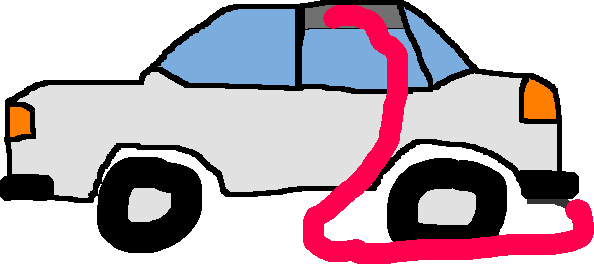
\includegraphics[width=0.5\textwidth]{Images/CarHeater.png}
				\caption[CarHeater]{When heating a car, the decision to rely on the implementation detail, that the catalytic converter removes all carbon monoxide from the exhaust gasses, usually yields results which are both dramatic and undesired. So it is preferable to stick to the documented features and use the car's heater.}
			\end{wrapfigure}
			Usually, there has been made at least a modest attempt to make the API versatile and easy to use and to document it sufficiently.
			And because APIs are so well thought through, they are unlikely to change.
			So when using a piece of software, it is reasonable to rely on the API and trust its documentation.
			All the aforementioned points mostly do not apply to the implementations behind APIs.
			That code tends to change regularly and its documentation is usually appalling, which provides unpromising conditions to depend on, when developing a software component.\\
			So take for example a function, whose documentation claims that it returns a unique identifier.
			When retrieving such an identifier, one can expect it to be unique, but all other assumptions are not valid, as they are not documented.
			Neither can one assume, that the identifier values are produced in the same order, after the program has been restarted.
			Nor is it allowed to make any assumptions about the type of the returned identifier.\\
			If one relies on internal details of an API implementation, the program will work at first, but it is very likely, that it will behave peculiarly, once this implementation has changed.
			Such errors are usually hard to find, as they often do not crash the program completely and the defective code is in a different area than the recent changes.

		\subsubsection{Explicit is better than implicit}
			This is one of the famous Python mantras.
			It basically means, that one should produce clean and readable code by avoiding implicit assumptions.
			The simplest example for this is passing arguments to a function as keyword arguments rather than positional arguments, when the number of arguments exceeds two.\\
			But this mantra also refers to API design.
			It is usually better to ask for every value explicitely, rather than guessing it from another source.
			A good example for this is the implementation of a class.
			A class should ask for every necessary parameter in its constructor, so that objects of that class are always fully initialized.\\
			If a parameter is not passed via the constructor, but later given via a setter method, the programmer of that class can decide between two evils.
			Either the object is not fully initialized, before that setter has been called, or the constructor tries to guess a reasonable value for that parameter.
			Such guessing code is usually messy, not documented and incapable of guessing always right, which will eventually result in an error.
			And, as the keen reader might have guessed by now, ''eventually'' is much worse in this context than ''always'', because such irregular errors are harder to find, to reproduce and it is more difficult to verify their absence through automated tests.\\
			The clean way would be to ask for that parameter in the constructor and give it a default value.
			Those default values are part of the API of a class, so it is specified explicitely, what value that parameter will have by default, rather than guessing the value implicitly.

		\subsubsection{Don't program a mathematical function yourself}
			Especially for Python, there are good libraries for almost any general problem available.
			So it is not necesseary to program something as general as a common mathematical function on one's own.\\
			With mathematical functions, the usual drawbacks of homebrew implementations are just suboptimal performance and maybe a bad API for that function.
			This is not good, but certainly not critical.\\
			The topic becomes more severe, when it comes to security relevant components like cryptography algorithms.
			Here it is absolutely mandatory, to use an open implementation, that has been reviewed and tested by as many people as possible.
			The ''security by obscurity'' approach of using a custom cryptography algorithm has nearly always proven to be insecure (and if there is an application, where it hasn't yet, it is just a matter of time until it does prove to be insecure...).

		\subsubsection{If in doubt, leave it out}
			If one is not sure, that a certain feature is needed, this feature should not be added to the software.
			After a feature has been introduced, there is nearly always a component or a user that relies on it and thus makes it impossible to remove it, even if the feature is faulty or deprecated.
			So adding a requested feature later on is usually easier than removing an unused feature, that one does not want to maintain anymore.


	\section{Mutable vs. Immutable data types}
		A mutable object is an object, whose data can be modified after the object has been fully initialized.
		Immutable objects on the other hand get all their data through their constructor and cannot be changed afterwards.\\
		Since immutable objects cannot be modified, processed versions of those objects have to be stored in new objects.
		In-place processing of an immutable object is not possible.\\
		The performance penalty for this is often far lower than expected, so choosing an object to be mutable, that could (or should) be immutable, might only be necessary on systems with extremely tight memory restrictions.
		Immutability also avoids the necessity to copy the object, each time it is passed to another part of the software, because the object cannot be modified unexpectedly and therefore passing a reference is sufficient.
		This usually gives tremendous speedups and much lower memory consumption compared to a mutable implementation.

		Generally, an object should be mutable, if the object is defined by its instance, rather than its data.
		A character in a computer game is still the same character, even after it has been moved to a different position (the position is part of the character object's data).
		So it is a sensible choice to make the character object mutable.

		If an object is only defined by its data, like for example a signal, it should be implemented as an immutable object.
		Consider the following example for an explanation why:
		\begin{minted}[gobble=3, tabsize=4]{python}
			# mutable
			loaded_signal = load_file(filename)
			normalize(loaded_signal)
			# immutable
			loaded_signal = load_file(filename)
			normalized_signal = normalize(loaded_signal)
		\end{minted}
		In the implementation, where signals are mutable objects, a signal is loaded from a file and then normalized in-place.
		This has the result, that the variable {\normalfont \ttfamily loaded\_signal} does not contain the signal that has been loaded from the file, as one would expect because of the name, but the normalized signal.
		This becomes especially dangerous, when the referene to the signal is passed to different parts of the software.\\
		In this case, it would be necessary to either copy the signal every time it is passed, or to assume that the signal is never processed.
		The copying solution costs a lot of memory and the copying is considerably slower than the passing of a reference.
		Doing without processing the signal will cripple the main functionality of the software (which is most likely signal processing) and if the signal is processed anyways, the poor programmer goes to debugging hell, because the program will not crash where the error has been made by modifying the signal, but at another part, where the signal is referenced.
		Maybe the program will not even crash, but just compute rubbish data, which is especially malicious, as it entrusts the detection of the error to the user.\\
		In the immutable implementation, the loaded and the normalized signal are stored in separate variables.
		And the references to the implementation can be passed to other parts of the software without the danger of unexpected modifications.

		The question of mutability is not only important for the implementation of classes.
		It must also considered for any other data that is passed through a programming interface, like arguments and return values of functions.
		So it is always recommended to use tuples instead of lists for such data.

		Returning data by calling a function with a reference to a mutable variable (return-by-call-by-reference) is a peculiar habit, that sprouted in the environment of software written in C.
		In C, this is the easiest way to return multiple values with one function.
		Furthermore, the explicit notation of pointers in C makes it obvious that the variable would be modified by the function call.\\
		In Python it is rather convenient to return multiple values with a tuple, while pointers are not exposed to the programmer.
		So it is absolutely not necessary for a function to have the side effect of modifying one of its parameters.
		If a mutable object shall be modified, it is cleaner to implement this modification in a method of its class, rather than an external function.
		This way, the method can encapsulate the implementation of the class, while an external function would rely on exposed internals of the class.


	\section{Global state}
		Global state is when mutable objects are accessible from several independent components of a software's source code.
		The problem with such objects is, that changing one of them has consequences, that reach beyond the scope of the current component.
		So the risk of undesired side effects is greatly increased.
		To cope with these side effects, it is usually necessary to perform extensive checks, when accessing such a global object.
		And when these checks fail, the resulting error is often hard to find and a lot of work to fix, because it involves many components of the software.

		When thinking about global state, one is usually reminded of global variables and that they are considered to be evil.
		They actually are, but also other malicious constructions exist, which create global state:
		\begin{itemize}
			\item Mutable singletons\footnote{Singletons are objects that are only instantiated once. When attempting to create another instance, one will only obtain the same instance, that was created before.}
			\item Modules (since they are singletons)
			\item File access
		\end{itemize}

		The classification of modules as harmful global state might need some explanation.
		Most modules just provide functionality and are not meant to be modified, which means, that they do not share state between the components which use the same module, so all is well.
		Other modules, like the {\normalfont \ttfamily atexit} module, do have functions, which change the state of that module, which requires some caution.
		In case of the {\normalfont \ttfamily atexit} module, this is usually not critical, as other software components are not affected, when one component registers a function, that shall be executed, when the program terminates.\\
		But there actually are negative examples for global state in modules.
		One of these is the {\normalfont \ttfamily random} module, which allows a reinitialization of the global random number generator with its {\normalfont \ttfamily seed} function.
		This design decision has probably been made, to facilitate the writing of simple scripts, but in more complex software, this function can easily be misused.
		For example, when one component seeds the generator with a special value and expects a specific sequence of generated random numbers (this assumption is reasonable, as the generated numbers are only ''pseudo random'', which means that their generation follows a deterministic law).
		If another component changes the state of the random number generator (e.g. by retrieving a number or by calling the global {\normalfont \ttfamily seed} function again), the assumptions of the first component about the generated sequence will be wrong.
		To circumvent this problem, one should always create a local instance of the random number generator ({\normalfont \ttfamily random.Random()}), when the actual values of the generated numbers are of importance.\\
		Another example of global state in modules is appending to {\normalfont \ttfamily sys.path}, which might be tolerable in trivial scripts, but is absolutely prohibited in even small software projects.

		File access is also a common source of errors due to global state.
		Especially with configuration files, it is likely, that different software components modify the same file, which can lead to race conditions or inconsistencies of loaded configuration parameters.
		So it is advised to encapsulate the access to a certain file in a single component, as this makes it easy to avoid race conditions.
		Furthermore, functions and classes should ask for all their parameters as arguments, rather than retrieving them from a global data source like the configuration.
		This encourages a software design, in which all external parameters are loaded only once (maybe at the beginning of the software's execution).

		There is even a more theoretical justification for avoiding global state, which has to do with provability.
		Consider the following logical conclusion as an example for this:
		\begin{equation}
			\left.
			\begin{aligned}
				A \Rightarrow B\\
				B \Rightarrow C
			\end{aligned}
			\right\} \Rightarrow \quad A \Rightarrow C
		\end{equation}
		This conclusion is only valid, when all objecs \(A\), \(B\) and \(C\) are the exactly the same throughout the whole set of formulas.
		This requirement seems trivial, but with global state, it is easy to dissatisfy, as the following piece of code shall demonstrate:
		\begin{minted}[gobble=3, tabsize=4]{python}
			threshold = 0	# a global variable
			def A(parameter):
				return parameter >= threshold
		\end{minted}
		When the value of the global variable changes, {\normalfont \ttfamily A} might still be the same instance, but from a mathematical point of view, it has become a different function, since it might yield a different result for the same parameter.
		So testing, if the software works correctly, becomes extremely hard, because theoretically all conclusions, that are drawn from the test runs, have to be validated for every possible combination of values for the global variables, which is usually impossible.\\
		The remedy for this problem is simply to make the global variable a parameter of the function.
		\begin{minted}[gobble=3, tabsize=4]{python}
			def A(parameter, threshold=0):
				return parameter >= threshold
		\end{minted}
		This way, the function always returns the same result for a given combination of arguments, so it remains the same function also in the mathematical sense.
		This allows it to test the function like a mathematical function, which can usually be done without brute force testing all possible parameter combinations.

		Functional programming languages like Haskell go to great lengths to avoid global state.
		This makes programming in such languages very counterintuitive for programmers, who are only familiar with imperative programming languages like Python.
		But since the lack of state makes functional programming languages very similar to mathematical formulas, it is much easier to apply the methods of proving mathematical theorems on programs in these languages.
		Sometimes it is even possible to formally prove the correctnes of a given implementation.


	\section{Design Patterns}
		Design patterns are generic solutions to problems, that occur regularly during the design and implementation of software.
		A surprising amount of research has been done to investigate the advantages and drawbacks of certain design patterns, so the established design patterns are often faster, easier to maintain and easier to extend than naive implementations.
		So it is always recommended to know the basic design patterns and to develop a feeling for recognizing, when such a pattern might be applicable.

		\subsection{The Observer Pattern}
			\label{ObserverPattern}
			The Observer Pattern is used, when one part of the software needs to retrieve data from another part, but does not know, when this data becomes available.

			Consider the example of a user interface, that wants to show the value of a sensor reading, but does not know, when the sensor is delivering new data.

			A naive solution would be simple polling:
			\begin{minted}[gobble=4, tabsize=4]{python}
				retrieved = 0.0
				while not timeout:
					new_value = sensor_driver.GetSensorReading()
					if new_value != retrieved:
						retrieved = new_value
						user_interface.Update(retrieved)
			\end{minted}
			It becomes immediately obvious, that this implementation calls the GetSensorReading-method far too often, which might result in a horrible performance of the software.

			A slightly more sophisticated (but even worse) solution would be to call the user interface's Update-method from the sensor driver.
			\begin{minted}[gobble=4, tabsize=4]{python}
				def OnNewSensorReading(new_value):
					"""
					This function is located in the sensor driver
					and processes the new value from the sensor.
					"""
					user_interface.Update(new_value)
			\end{minted}
			Compared to the polling implementation, this implementation reverses the dependencies, by making the sensor driver depend on the user interface, while a user interface could be instantiated without a sensor driver.
			The advantage of this implementation is, that all necessary information is available in the sensor driver; it knows the value of the sensor reading, it knows the time when the reading changes, and it knows about the user interface, that wants to do something with the sensor value.
			This way, it is possible to do without polling and the performance penalty that comes with it.\\
			The drawback of this implementation is that the order of dependencies is now very peculiar and counterintuitive, which will lead to a non-extensible and unmaintainable codebase.
			The user interface, which has the purpose of displaying sensor results, can now be instantiated without specifying any sensors, which does not make sense, but it is at least not dangerous.
			A sensor driver, on the other hand, can now only be instantiated with a specified user interface, which leads to an infinte wealth of problems.\\
			The sensor driver can no longer be instantiated without a user interface, which makes automated testing of the driver almost impossible.
			If many different sensors are used (which is likely), the update of the user interface has to be implemented in every single one of them.
			If the user interface changes (which is likely), every single driver has to be adapted to these changes.
			If the sensor drivers shall be used for a similar software, that writes the sensor readings into a data base instead of displaying it in a user interface, the already available drivers cannot be reused, because they are only for updating a user interface.
			If the user interface raises an error (which is likely, because testing user interfaces is hard), the crash also affects the sensor driver, which can make debugging a nightmare.\\
			In essence, this implementation is a clear violation of the ''Do only one thing and do it well''-paradigma.
			The update of the user interface must not be a responsibility of such a low level part as a sensor driver.

			The Observer Pattern offers a much more elegant solution, that does without polling, but keeps the sensor driver independent of the user interface.
			This avoids all drawbacks of the aforementioned implementations at the cost of a slightly higher programming effort.\\
			The idea of the Observer Pattern is, that a part of a software, that wants to be notified about an event (like a new sensor value), passes a callback object to the part of the software, that generates the event.
			This way, the event generating part has all necessary information to handle the event properly, so polling is not necessary.
			In addition, the event generating part does not depend on any other parts of the software, as it can just discard the event, if no callback objects are specified.

			The following code shows a rudimentary implementation of the sensor-user-interface-example, that uses the Observer Pattern:
			\begin{minted}[gobble=4, tabsize=4]{python}
				class UserInterface(object):
					def __init__(self, sensors):
						for s in sensors:
							# inform all sensors that the user
							# interface wants to be notified
							s.AddObserver(self.Update)

					def Update(self, sensor, sensor_value):
						print("Sensor %s has new value: %f" % (str(sensor), sensor_value))

				class SensorDriver(object):
					def __init__(self):
						self.__observers = []
				
					def AddObserver(self, callback):
						"""
						Stores the given callback functions
						"""
						self.__observers.append(callback)

					def OnNewSensorReading(new_value):
						"""
						Is magically called, when a new sensor reading is available
						"""
						for o in self.__observers:
							# notify all interested program parts
							# by calling every callback object
							o(self, new_value)

				sensor = SensorDriver()
				user_interface = UserInterface(sensors=[sensor])
			\end{minted}
			If many sensor drivers have to be implemented, the programming overhead of the Observer Pattern can be reduced, by sharing the necessary code trough inheritance.
			The advantages of this implementation become obvious, when the performance, the maintenance and possible extensions are considered:
			\begin{itemize}
				\item No polling
				\item A sensor driver can be instantiated and tested without any observing object
				\item Adding a new front end (like a data base that stores the sensor data) requires no changes in the sensor drivers' code
				\item It is even possible to use multiple front ends simultaneously (user interface and data base, maybe even more) without changing the sensor drivers
			\end{itemize}

			When the observing objects (in the example, this is the user interface) are destroyed, it is necessary to delete the callbacks that have been passed to the AddObserver-method aswell.
			So it is required to implement a RemoveObserver-method aswell.
			\begin{minted}[gobble=4, tabsize=4]{python}
				class SensorDriver(object):
					...
					def RemoveObserver(self, callback):
						self.__observers.remove(callback)
					...
			\end{minted}
			Due to the very dynamic nature of Python, it is necessary to generate new objects from the methods in certain cases.
			Therefore it is not guaranteed, that different references to the same method (in the example self.Update) link to the same object, which is a mandatory requirement for the lists remove-method (as used in the RemoveObserver-method) to work.
			This pitfall can be avoided by storing a weak reference to the method and passing that to the AddObserver- and RemoveObserver-methods.
			It has to be a weak reference, so the automatic deletion of unused objects is not annulled by circular references (more on this in Chapter~\ref{PythonPitfalls} about the common pitfalls when using Python).
			\begin{minted}[gobble=4, tabsize=4]{python}
				import weakref

				class UserInterface(object):
					def __init__(self, sensors):
						self.__update_method = weakref.proxy(self.Update)
						for s in sensors:
							s.AddObserver(self.__update_method)
					...
			\end{minted}


		\subsection{Other Patterns}
			The Observer Pattern is so cool, you can conquer the world just with that.
			But still, some more patterns would be helpful, so: TODO

